%!TEX root = slides.tex

\section{Languages}

\begin{frame}{Popular programming languages}
  \begin{description}
    \item[JavaScript] ``high-level, dynamic, untyped, and interpreted''
    \item[SQL] ``special-purpose programming language''
    \item[Java] ``general-purpose, concurrent, class-based, object-oriented''
    \item[C\#] ``multi-paradigm programming language''
    \item[PHP] `` server-side scripting''
    \item[Python] ``high-level, general-purpose, interpreted, dynamic''
    \item[C++] ``general-purpose, imperative, object-oriented and generic''
    \item[C] ``general-purpose, imperative''
    \item[Others] Node.js, AngularJS, Ruby, Objective-C (in order).
  \end{description}
  \citeurl{http://stackoverflow.com/research/developer-survey-2016}
\end{frame}


\begin{frame}{Kinds of programming languages}
  \begin{description}
    \item[Interpreted] Software interprets the language at runtime. 
    \item[Compiled] Software translates the language into machine code, which is then run.\\[1cm] 
    \item[Systems] Designed with operating system, device drivers development in mnid.
    \item[Applications] Designed with user applications development in mind.\\[1cm]
    \item[High-level] Abstration from the nitty-gritty computer details.
    \item[Imperative] Statements change the program state.
  \end{description}
\end{frame}

\begin{frame}{New languages}
  \begin{description}
    \item[Go] 2009 at Google. 
    \item[Rust] 2010 at Mozilla.
    \item[Swift] 2014 at Apple.
    \item[Hack] 2014 at Facebook, variant of PHP.
    \item[Scala] 2004 at EPFL (Martin Odersky).
    \item[Julia] 2012 at MIT.
    \item[Dart] 2011 at Google.
  \end{description}
\end{frame}


\begin{frame}{Styles in languages}
  \begin{figure}
    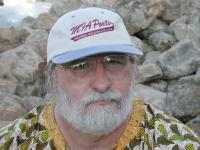
\includegraphics[height=3cm]{img/richard-gabriel.jpg}
  \end{figure}
  \begin{quote}
    I'm always delighted by the light touch and stillness of early programming languages.
    Not much text; a lot gets done.
    Old programs read like quiet conversations between a well-spoken research worker and a well studied mechanical colleague, not as a debate with a compiler.
    Who'd have guessed sophistication bought such noise? \\
    \hspace*\fill{\small--- Dick Gabriel}
  \end{quote}

  \citeurl{web.stanford.edu/class/ee380/Abstracts/100428-pike-stanford.pdf}
\end{frame}

\begin{frame}{People: Dennis Ritchie}
  \begin{figure}
    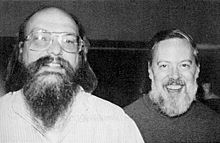
\includegraphics[height=3cm]{img/ritchie-thompson.jpg}
    \caption*{Dennis Ritchie 1941-2011 (right)}
  \end{figure}
  \begin{itemize}
    \item Helped Ken Thompson (left in above photo) to create UNIX.
    \item Created C, wrote book with Brian Kernighan.
  \end{itemize}
\end{frame}

\begin{frame}{People: Ken Thompson}
  \begin{figure}
    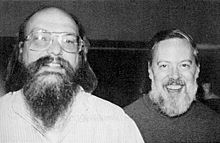
\includegraphics[height=3cm]{img/ritchie-thompson.jpg}
    \caption*{Ken Thompson (left)}
  \end{figure}
  \begin{itemize}
    \item Created UNIX.
    \item One of the creators of Go.
  \end{itemize}
\end{frame}


\begin{frame}{People: Brian Kernighan}
  \begin{figure}
    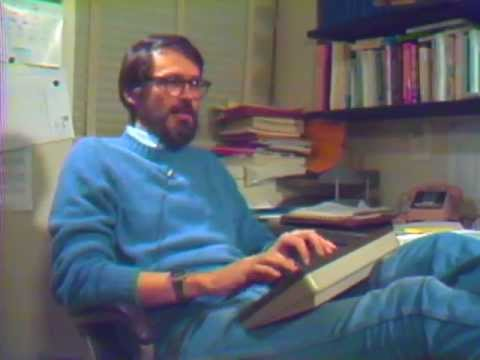
\includegraphics[height=3cm]{img/brian-kernighan.jpg}
  \end{figure}
  \begin{itemize}
    \item Wrote \emph{The C Programming Language} with Dennis Ritchie.
    \item Coined \mintinline{c}{Hello, world!}.
    \item Wrote \emph{The Go Programming Language} (with Alan Donovan).
  \end{itemize}
\end{frame}

\begin{frame}{People: Bjarne Stroustrup}
  \begin{figure}
    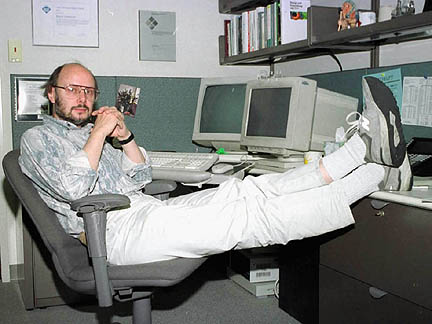
\includegraphics[height=3cm]{img/bjarne-stroustrup.jpg}
  \end{figure}
  \begin{itemize}
    \item Created C++.
    \item Former head of Large-scale Programming Research at Bell Labs.
  \end{itemize}
\end{frame}

\begin{frame}{Places: Bell Labs}
  \begin{figure}
    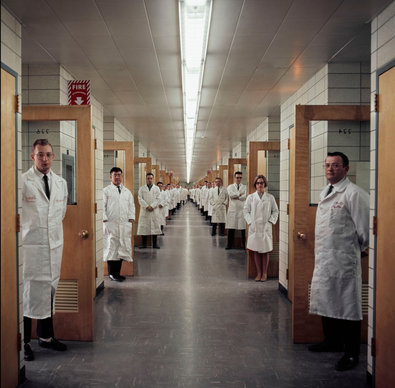
\includegraphics[height=3cm]{img/bell-labs.jpg}
  \end{figure}
  \begin{itemize}
    \item Pretty much set up by Alexander Graham Bell.
    \item Eight Nobel prizes, two Turing awards.
    \item Owned by Alcatel-Lucent, who were bought by Nokia.
  \end{itemize}
\end{frame}